\documentclass{ieeeojies}
\usepackage{cite}
\usepackage{amsmath,amssymb,amsfonts}
\usepackage{algorithmic}
\usepackage{graphicx}
\usepackage{textcomp}
\usepackage{array}
\usepackage[table]{xcolor}
\usepackage{multirow}
\usepackage{multicol}
\usepackage{float}
\usepackage{hyperref}
\usepackage{indentfirst}

\setlength{\parindent}{0.5cm}
\def\BibTeX{{\rm B\kern-.05em{\sc i\kern-.025em b}\kern-.08em
    T\kern-.1667em\lower.7ex\hbox{E}\kern-.125emX}}

\begin{document}
\title{FORECASTING STOCK PRICES IN VIETNAM USING MACHINE LEARNING AND DEEP LEARNING MODELS}

\author{\uppercase{Tran Truc Quynh}\authorrefmark{1},
\uppercase{Luong Thi Thuy Diem\authorrefmark{2}, and Nguyen Huu Thanh}\authorrefmark{3}}

\address[1]{Faculty of Information Systems, University of Information Technology, (e-mail: 21522539@gm.uit.edu.vn)}
\address[2]{Faculty of Information Systems, University of Information Technology, (e-mail: 21521953@gm.uit.edu.vn)}
\address[3]{Faculty of Information Systems, University of Information Technology, (e-mail: 21522599@gm.uit.edu.vn)}

\markboth
{Author \headeretal: Tran Truc Quynh,Nguyen Huu Thanh,Luong Thi Thuy Diem}
{Author \headeretal: Tran Truc Quynh,Nguyen Huu Thanh,Luong Thi Thuy Diem}

\begin{abstract}
The stock market has assumed a significant position within investment portfolios, as evidenced by the recent surge in investor participation within Vietnam's market. However, navigating the inherent volatility of stock prices requires experience and robust analytical tools. This paper seeks to empower investors by employing various forecasting models such as Linear Regression (LR), Auto Regressive Integrated Moving Average (ARIMA), ecurrent neural network (RNN), Gated Recurrent Units (GRU),Long short term memory (LSTM), Fast Fourier Transform (FFT),XGBOOST, Fully Convolutional Networks (FCNs) to analyze price trends within three prominent bank stocks: ACB, BIDV, VCB traded on Hochiminh Stock Exchange (HOSE) over a five-year period (2019-2024). By evaluating the effectiveness of these models using RMSE, MAPE, and MSLE techniques. This paper aims to equip investors for informed stock selection within their portfolios, ultimately contributing to more accurate decision-making.
\end{abstract}

\begin{keywords}
Time Series Analysis, Machine Learning, Financial Forecasting, Vietnamese Stock Market,
GRU, RNN, ARIMA, LSTM, FFT, XGBoost, FCN, Linear Regression.
\end{keywords}

\titlepgskip=-15pt

\maketitle

\section{Introduction}
\label{sec:introduction}

The Vietnamese stock market has witnessed a record-high level of participation in recent years, reflecting the growing attention and interest it has garnered. This trend is a positive indicator of the market's potential and the overall recovery of the economy in the post-2023 period. However, the stock market also inherently carries short-term risks that investors must navigate. Among the various sectors, the banking industry has traditionally occupied a high proportion and serves as a crucial pillar of the economy.

The purpose of this paper is to support investors in making accurate decisions regarding three bank stocks (ACB, BID, VCB) listed on the Hochiminh Stock Exchange (HOSE).
To achieve this goal, the study will apply various models, including Linear Linear Regression (LR), Auto Regressive Integrated Moving Average (ARIMA), ecurrent neural network (RNN), Gated Recurrent Units (GRU),Long short term memory (LSTM), Fast Fourier Transform (FFT),XGBOOST, Fully Convolutional Networks (FCNs) to the stock price data from 2019 to 2024 to forecast the trends.Techniques such as RMSE, MAPE, and MSLE will be utilized to evaluate the effectiveness of these models.
\section{Related Works}
Over the past several years, a significant volume of research has concentrated on forecasting stock prices by leveraging various machine learning and statistical techniques. Both CAKRA (2015) and URAS (2020) used linear regression to forecast stock prices and Bitcoin closing prices. CAKRA applied linear regression based on sentiment analysis to process Twitter data, improving the accuracy of stock price predictions \cite{cakra2015stock}. Meanwhile, URAS combined linear regression and neural network models to forecast Bitcoin closing prices, showing that linear regression had faster execution speed and could accurately predict Bitcoin price fluctuations \cite{uras2020forecasting}.\\

Manish Dadhich studied and applied the ARIMA model for short-term forecasting of BSE and NSE stock prices. After carrying out his research, Manish Dadhich demonstrated the strength of the ARIMA model in predicting daily closing prices of time series data \cite{dadhich2021predictive}. In Anusha Garlapati's research, she also used ARIMA to forecast stock prices and concluded that ARIMA is a good model for predicting stock prices \cite{garlapati2021stock}.\\ 

Yongqiong Zhu \cite{ZhuRNN} applied an RNN model to predict the stock prices of Apple. The training dataset spanned 10 years with 65\% allocated for training and the remaining 3\% for testing. With 50 epochs, Adam optimization, and Mean Squared Error (MSE) as the loss function, the model achieved highly favorable outcomes. It attained a predictive accuracy exceeding 95\%, with a reported loss value of 0.1\%. In 2015, Xiao Ding \cite{DingGRU} also proposed a deep learning method for event-driven stock market prediction.\\

Shejul et al. \cite{ShejulGRU} compared the performance of the Gated Recurrent Unit (GRU) and Bidirectional Long Short-Term Memory (BiLSTM) models in predicting stock prices. Experimental results indicate that both models accurately forecast future stock prices, with the BiLSTM model outperforming the GRU model. Despite this, the GRU model demonstrates nearly double the speed of the BiLSTM model due to its simpler architecture. Overall, both models offer precise predictions and can effectively anticipate future stock market trends.\\

C. Fjellström (2022) \cite{fjellstrom2022lstm} explored an LSTM ensemble for stock price prediction in the paper "Long Short-Term Memory Neural Network for Financial Time Series." The work demonstrates superior performance over traditional portfolios, offering insights into LSTM's potential for financial forecasting and strategies for enhancing model accuracy and reducing market risk. S. Mehtab, J. Sen (2020) \cite{mehtab2020stock} proposed a deep learning approach for stock price prediction by employing Convolutional Neural Networks (CNN) and Long Short-Term Memory (LSTM) networks. Their work contributes to the field by exploring the effectiveness of this combined deep learning architecture in forecasting the NIFTY 50 index prices. They further emphasize the importance of data pre-processing and model evaluation, providing a methodological blueprint for financial market analysis using deep learning techniques.\\

Chen et al.\cite{ChenFFT} used an Fast Fourier Transform algorithm to deal with historical training data for forecasting stock prices, achieving a more highly accurate. Experimental analysis is performed on datasets covering a seven-year period of both the Taiwan Stock Exchange Capitalization Weighted Stock Index (TAIEX) and the Dow-Jones Industrial Average (DJIA). \\

A. Qingwen Jin et al. \cite{jin2019using} established predictive models using the Best Track TC dataset and the XGBOOST algorithm to anticipate Tropical Cyclone (TC) intensity in the Western North Pacific (WNP). Across six scenarios, the model achieved high accuracy with MAE < 4.50 m/s, CC > 0.89, and NRMSE < 10.00\%. The XGBOOST model exhibited superior performance compared to traditional Back-Propagation Neural Network (BPNN) models for the same predictors and independent prediction samples. A. O. A. A. A. Tianqi Chen and Carlos Guestrin (2016)\cite{chen2016xgboost} introduced XGBoost, a scalable tree boosting system. The paper describes the architecture of XGBoost and its core algorithms, presenting improvements to enhance performance and accuracy across a variety of machine learning tasks.\\

Fully Convolutional Networks (FCNs) have been studied and applied in various fields related to image data processing and semantic segmentation. According to Shima Nabiee's research on stock trend prediction, FCNs have also been proven to be a powerful and flexible tool, enabling the analysis and prediction of stock price trends based on raw data \cite{nabiee2023stock}.
\section{Materials}
\subsection{Dataset}

The analysis will focus on the historical stock prices of three banks in Vietnam: the Asia Commercial Joint Stock Bank (ACB), the Bank for Investment and Development of Vietnam (BIDV), and the Joint Stock Commercial Bank for Foreign Trade of Vietnam (VCB). The data spans from January 3, 2019, to January 3, 2024, and includes information such as date, price, opening price, highest and lowest prices, volume, and price change. However, the primary aim is to forecast closing prices, so only the "Price" column (VND) will be used for analysis.

\subsection{Descriptive Statistics}
\begin{table}[H]
  \centering
  \caption{ACB, BIDV, VCB’s Descriptive Statistics}
  \begin{tabular}{|>{\columncolor[HTML]{4CCD99}}c|c|c|c|}
    \hline
     \rowcolor[HTML]{4CCD99} & ACB & BID & VCB \\ \hline
     Count & 1247 & 1252 & 	1252 \\ \hline
     Mean & 19.712	 & 35.993 & 74.810\\ \hline
     Standard Deviation  & 6.205 & 6.574 & 12.664\\ \hline
     Min & 8.763 & 23.420 & 43.925\\ \hline
     25\% & 11.963 & 31.226 & 65.274\\ \hline
     50\% & 22.000 & 34.823 & 75.871\\ \hline
     75\% & 24.980 & 41.600 & 84.525\\ \hline
     Max & 30.360 & 53.900 & 106.500\\ \hline
     Variance & 49.100 & 28.667 & 106.500\\ \hline
     Skewness & -0.345 & 0.299 & -0.132\\ \hline
     Kurtosis & -1.457 & -0.821 & -0.530\\ \hline
\end{tabular}
\end{table}
\subsubsection{ACB stock price visualization}
\begin{figure}[H]
    \centering
    \begin{minipage}{0.23\textwidth}
    \centering
    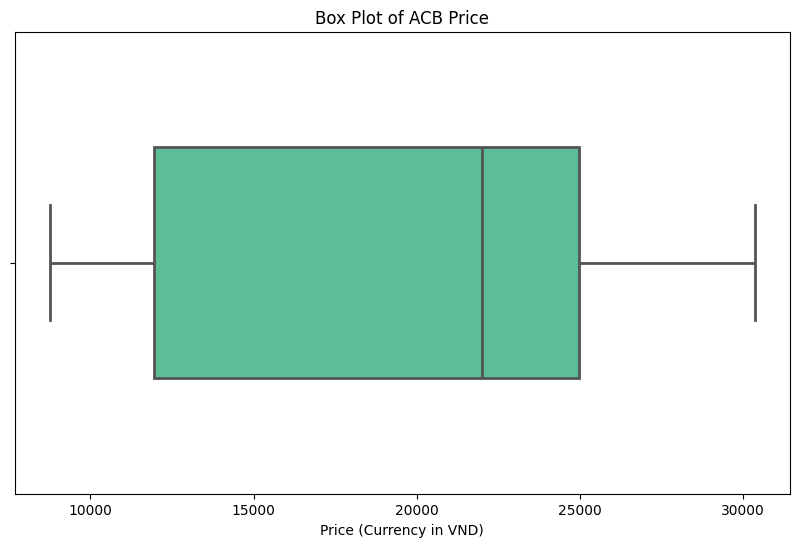
\includegraphics[width=1\textwidth]{bibliography/Figure/ACBboxplot.png}
    \caption{ACB stock price's boxplot}
    \label{fig:1}
    \end{minipage}
    \hfill
     \begin{minipage}{0.23\textwidth}
        \centering
        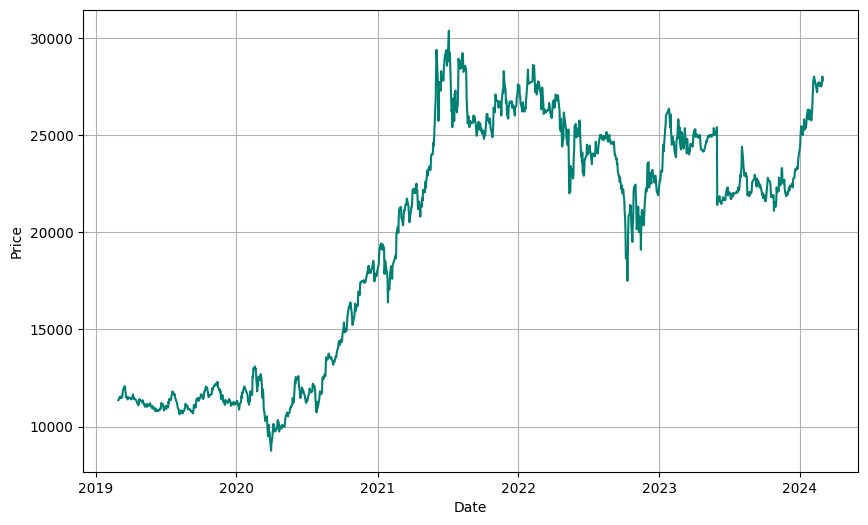
\includegraphics[width=\textwidth]{bibliography/Figure/ACBtime.png}
        \caption{ACB stock price's time}
        \label{fig:2}
    \end{minipage}
        \centering
    \begin{minipage}{0.23\textwidth}
    \centering
    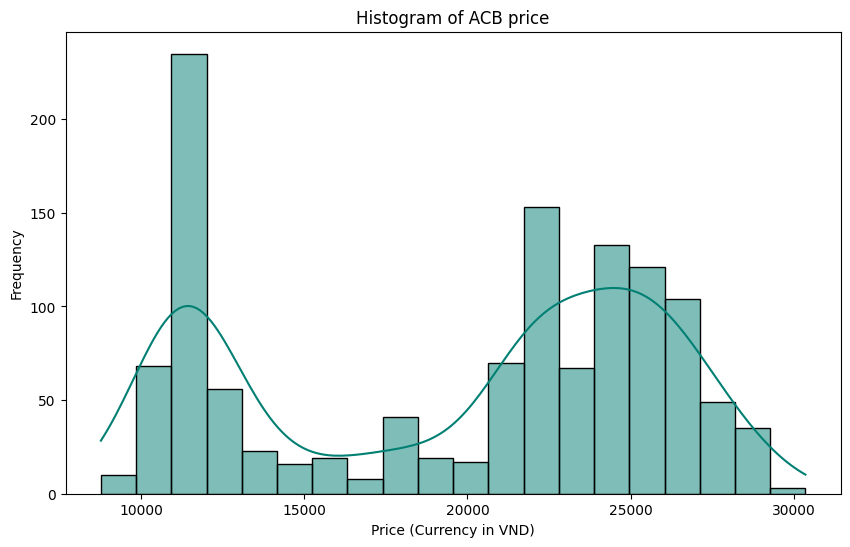
\includegraphics[width=1\textwidth]{bibliography/Figure/ACBhist.png}
    \caption{ACB stock price's histogram}
    \label{fig:3}
    \end{minipage}
\end{figure}
    ACB's price distribution appears left-skewed, as evidenced by the pronounced peak in the histogram at the lower end of the price range. Interestingly, ACB's box plot appears relatively compact, with the median closer to the higher end of the price range
\subsubsection{BID stock price visualization}
\begin{figure}[H]
    \centering
    \begin{minipage}{0.23\textwidth}
        \centering
        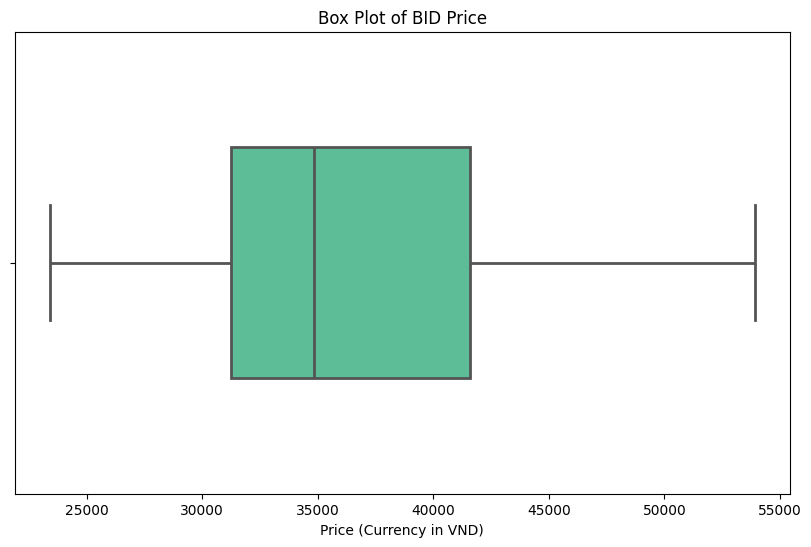
\includegraphics[width=1\textwidth]{bibliography/Figure/BIDboxplot.png}
        \caption{BID stock price's boxplot}
        \label{fig:1}
    \end{minipage}
    \hfill
    \begin{minipage}{0.23\textwidth}
        \centering
        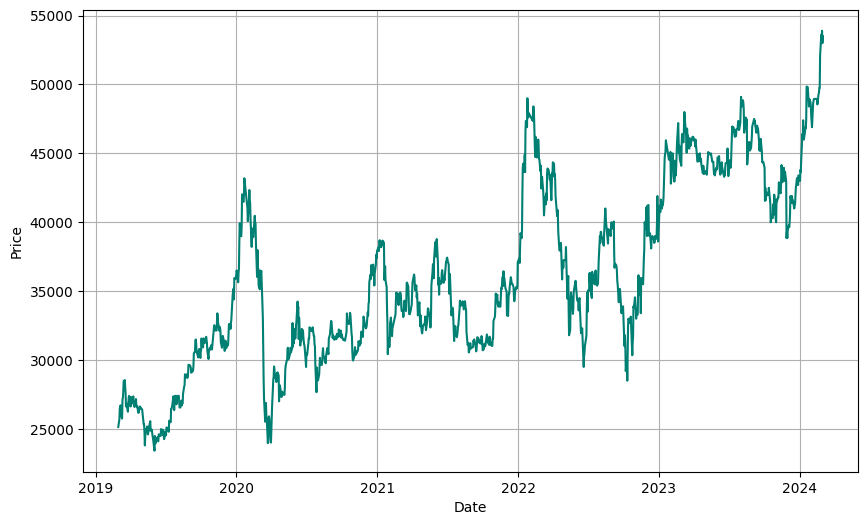
\includegraphics[width=\textwidth]{bibliography/Figure/BIDtime.png}
        \caption{BID stock price's time}
        \label{fig:2}
    \end{minipage}
    \begin{minipage}{0.23\textwidth}
        \centering
        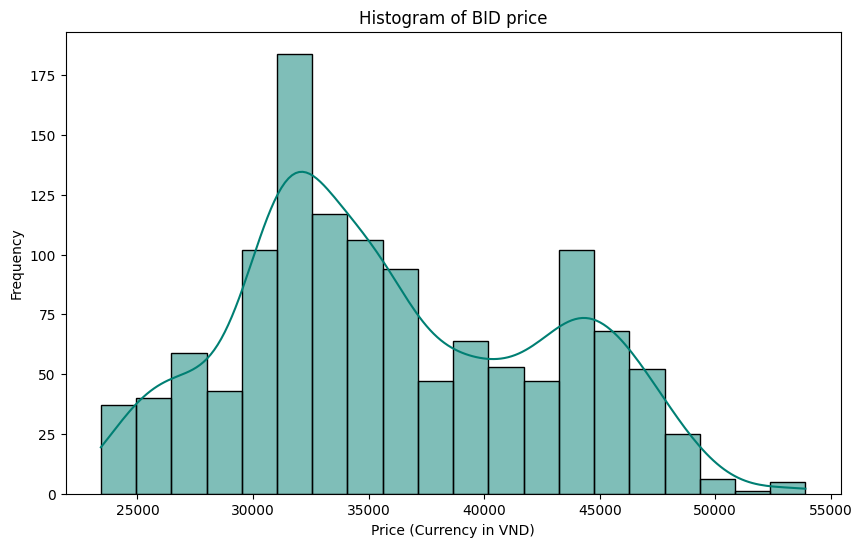
\includegraphics[width=1\textwidth]{bibliography/Figure/BIDhist.png}
        \caption{BID stock price's histogram}
        \label{fig:3}
    \end{minipage}
\end{figure}
The value of BID shares mainly fluctuates between 33,000 VND and 43,000 VND, and the highest current value that BID shares have reached is 54,000 VND. Additionally, the current trend regarding the value of BID shares is on the rise.
\subsubsection{VCB stock price visualization}
\begin{figure}[H]
    \centering
    \begin{minipage}{0.23\textwidth}
        \centering
        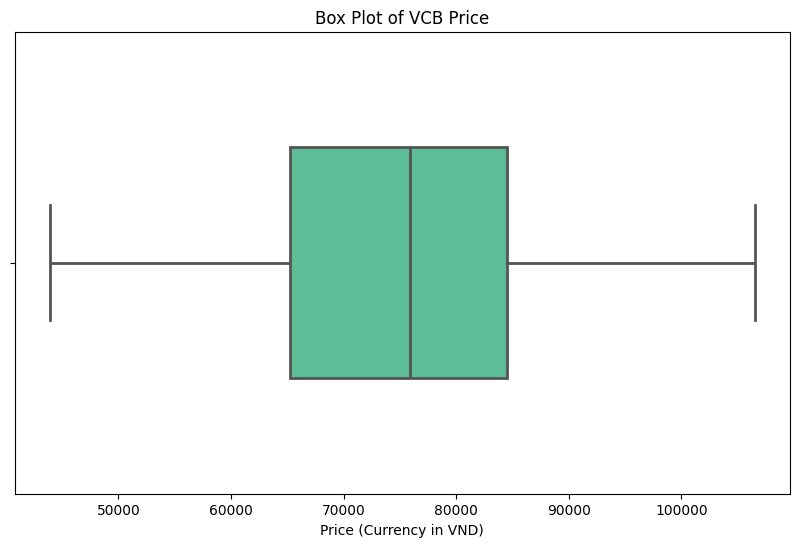
\includegraphics[width=1\textwidth]{bibliography/Figure/VCBboxplot.png}
        \caption{VCB stock price's boxplot}
        \label{fig:1}
    \end{minipage}
    \hfill
    \begin{minipage}{0.23\textwidth}
        \centering
        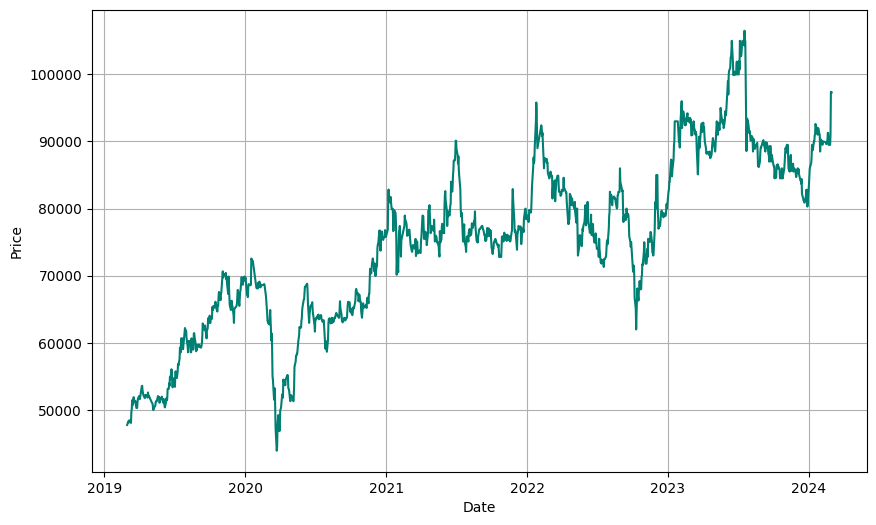
\includegraphics[width=1.1\textwidth]{bibliography/Figure/VCBtime.png}
        \caption{VCB stock price's time}
        \label{fig:2}
    \end{minipage}
    \begin{minipage}{0.23\textwidth}
        \centering
        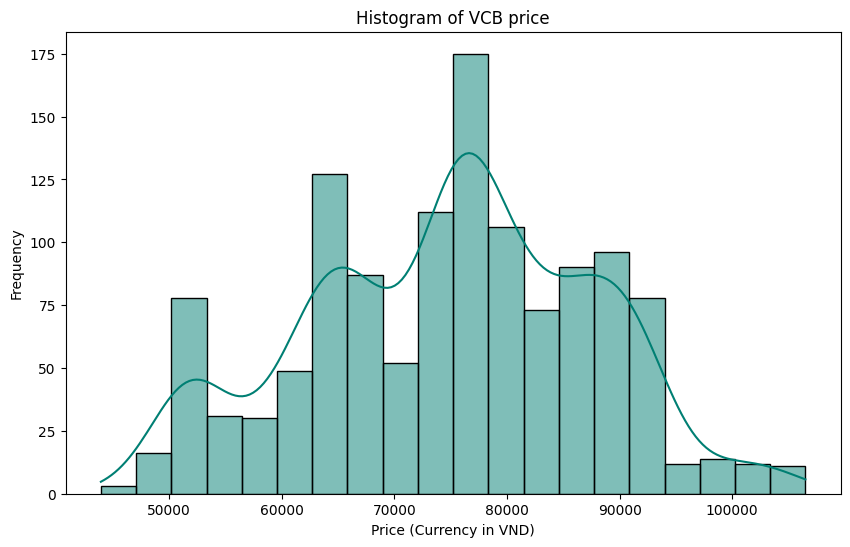
\includegraphics[width=\textwidth]{bibliography/Figure/VCBhist.png}
        \caption{VCB stock price's histogram}
        \label{fig:3}
    \end{minipage}
\end{figure}

% vcb boxplot
 Based on VCB's Boxplot, it can be seen that most of the data is concentrated in Q2 to Q3 with length 8654 approximately 75871 to 84525.
% vcb histogram
The highest concentration on the chart at the price of about 76,000 VND with a frequency of nearly 175 times may be a sign of investors' special interest in VCB stock price. Besides, the price also fluctuates frequently around 70,000
The data chart of price fluctuations over the years shows that stock prices tend to gradually increase, although prices also decrease to the lowest (43925) in early 2020 and the highest (106500) in mid-2023.
\section{Methodology}

\subsection{ARIMA}
Auto Regressive Integrated Moving Average (ARIMA) is a model that describes time series based on observed values, which can be used to forecast future values. Applying ARIMA models to any time series showing patterns with no random white noise and non-seasonality. The model was introduced by Box and Jenkins in 1970. To generate short-term forecasts, ARIMA models have shown efficient capabilities, outperforming complex structural models. The future value of a variable in the ARIMA model is a combination of linearity to the past values and errors, expressed as follows \cite{Gillian}:

\begin{equation*}
Y_t = \phi_0 + \phi_1 Y_{t-1} + \phi_2 Y_{t-2} + \ldots + \phi_p Y_{t-p} + \varepsilon_t - \theta_1 \varepsilon_{t-1} - \ldots - \theta_q \varepsilon_{t-q}
\end{equation*}

Where:
\begin{itemize}
    \item $Y_t$ is the actual value at time $t$.
    \item $\varepsilon_t$ is the random error at time $t$.
    \item $\phi_i$ and $\theta_j$ are the coefficients.
    \item $p$ and $q$ are integers, often referred to as autoregressive and moving average parameters, respectively.
\end{itemize}

\subsection{FAST FOURIER TRANSFORM}
The Fast Fourier Transform (commonly abbreviated as
FFT) is a fast algorithm for computing the discrete Fourier
transform (DFT) of a sequence \cite{Gillian} by using the factor N/2
log N where N is the number of points, therefore, the FFT is a
way to convert the time series from time domain to frequency
domain \cite{Musbah} with equation \cite{Roberts}: 
\[
F[n] = \sum_{k=0}^{N-1} f[k] \cdot e^{-i \frac{2\pi}{N} kn}
\]

where:
\begin{itemize}
    \item $F[n]$ is the Discrete Fourier Transform of the sequence.
    \item $f[k]$ is the $k$-th element of the input sequence.
    \item $N$ is the total number of elements in the input sequence.
    \item $n$ is the index of the frequency component in the output sequence $F[n]$.
    \item $k$ is the index of the element in the input sequence $f[k]$.
\end{itemize}

% Linear
\subsection{Linear Regression}
Linear regression is a statistical technique used to model the relationship between a dependent variable, \textit{Y}, and one or more independent variables, \textit{X}. The goal is to find the best-fitting straight line (or hyperplane in higher dimensions) that describes the relationship between the variables. 
When there are multiple independent variables, the linear regression is called multivariable linear regression, with equation has the form \cite{busin}:
 \[Y=\beta_0+\beta_1X_1+\beta_2X_2+\cdots+\beta_kX_k+\varepsilon\]
Where:\\
	\indent\textbullet\ Y is the dependent variable.\\
	\indent\textbullet\ \(X_1, X_2, \ldots, X_k\) are the independent variables.\\
	\indent\textbullet\ \(\beta_0\) is the intercept term.\\
	\indent\textbullet\ \(\beta_1,..., \beta_k\) are the regression coefficients for the independent variables.\\
	\indent\textbullet\ \(\varepsilon\) is the error term.

\subsection{XGBoost}
XGBoost is a highly efficient and scalable implementation of gradient boosting, a powerful machine learning technique. XGBoost operates by constructing a series of decision trees in an additive manner. Each tree is built sequentially, with each one correcting the errors of the previous trees. The model’s objective is to minimize the loss function. Key advantages of XGBoost include its ability to handle large datasets through parallelized computing, effective handling of missing data values, and flexible parameter tuning. These features, along with its state-of-the-art algorithm for supervised learning problems, known for its high accuracy, which rivals deep learning models\cite{Xgboost} .Unlike deep learning that typically requires numerical raw data, XGBoost can handle tabular datasets of any size and type, including categorical data often found in business models.  

Explanation of the mathematics behind XGBoost:\\
\textbf{Ensemble Model:}XGBoost combines predictions from multiple decision trees $(f_k)$ to create a final prediction (F(x))\cite{Xgboost}:
\begin{equation*}
y_i = \phi(x_i) = \sum_{k=1}^K f_k(x_i), \quad f_k \in \mathcal{F},
\end{equation*}

Where: $F = {f(x) = w_q(x) \mid q : \mathbb{R}^m \to T, w \in \mathbb{R}^T}$\\

\textbf{Objective Function:}
It minimizes a loss function (L) that measures prediction error, with a regularization term ($\Omega$) to prevent overfitting:\cite{geekXGboost}

\begin{equation*}
\text{obj}(\theta) = \sum_{i=1}^n l(y_i, \hat{y}_i) + \sum_{k=1}^K \Omega(f_k)
\end{equation*}

Where, first term is the loss function and the second is the regularization parameter\\

\subsection{GRU}
The Gated Recurrent Unit, just like the LSTM, is a Recurrent
Neural Network. It, however, has a less complicated structure
compared to LSTM. It lacks an output gate but has an update z
and a reset gate r. These gates are vectors which decide what
information should be passed to the output. 
The Reset gate defines how to combine the new input with the
previous memory. The definition of how much of the last memory
to keep is done by the Update [12]. The GRU has the following
equations:\cite{Yamak}
\\
Update gate:
\begin{equation}
z_t = \sigma(W_z h_{t-1} + U_z x_t)
\end{equation}
Reset gate:
\begin{equation}
r_t = \sigma(W_r h_{t-1} + U_r x_t)
\end{equation}
Cell state:
\begin{equation}
c_t = \tanh(W_c (h_{t-1} \ast r_t) + U_c x_t)
\end{equation}
New state:
\begin{equation}
h_t = (z_t \ast c_t) + ((1 - z_t) \ast h_{t-1})
\end{equation}
\begin{figure}[H]
    \centering
\begin{minipage}{0.5\textwidth}
        \centering
        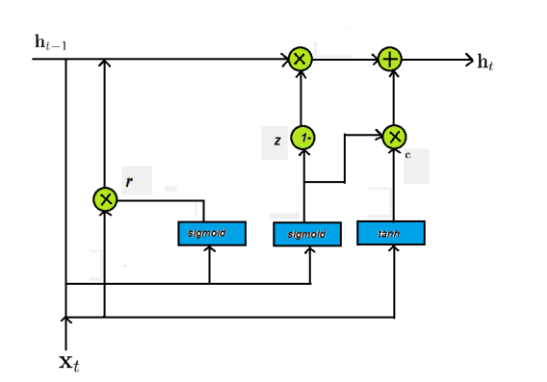
\includegraphics[width=\textwidth]{bibliography/Figure/GRU_diagram.png}
        \caption{Fully Convolutional Neural Network architecture}
        \label{fig:3}
\end{minipage}
\end{figure}

\subsection{Fully Convolutional Neural Network(FCN)}
Fully Convolutional Neural Networks (FCNs) were introduced by Wang et al. (2017b) for univariate time series classification, validated on 44 UCR/UEA datasets. FCNs use convolutional layers without local pooling, maintaining the time series length throughout. A key feature is replacing the final fully connected layer with a Global Average Pooling (GAP) layer, reducing parameters and enabling Class Activation Mapping (CAM) to identify crucial input segments. 
FCNs lack pooling and regularization, benefiting from parameter invariance across varying time series lengths due to GAP, supporting transfer learning for model adaptation from one dataset to another.\cite{Ismail}

\begin{figure}[H]
    \centering
\begin{minipage}{0.5\textwidth}
        \centering
        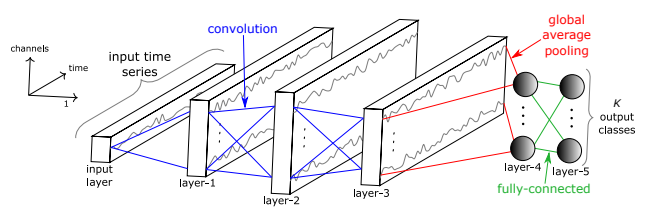
\includegraphics[width=\textwidth]{bibliography/Figure/FCN.png}
        \caption{Fully Convolutional Neural Network architecture}
        \label{fig:3}
\end{minipage}
\end{figure}
<<<<<<< HEAD
\subsection{Recurrent neural network (RNN)}
A recurrent neural network (RNN) is a type of artificial neural network which uses sequential data or time series data\cite{IBM}.  A recurrent neural network (RNN) is an extension of a conventional feedforward neural network, which is able to handle a variable-length sequence input. The RNN handles the variable-length sequence by having a recurrent hidden state whose activation at each time is dependent on that of the previous time\cite{Chung}.
For each timestep \( t \), the activation \( a^{<t>} \) and the output \( y^{<t>} \) are expressed as follows:
\[
a^{<t>} = g_1\left( W_{aa} a^{<t-1>} + W_{ax} x^{<t>} + b_a \right)
\]
and
\[
y^{<t>} = g_2\left( W_{ya} a^{<t>} + b_y \right)
\]
where \( W_{ax}, W_{aa}, W_{ya}, b_a, b_y \) are coefficients that are shared temporally and \( g_1, g_2 \) are activation functions \cite{standford}.

\begin{figure}[H]
    \centering
\begin{minipage}{0.5\textwidth}
        \centering
        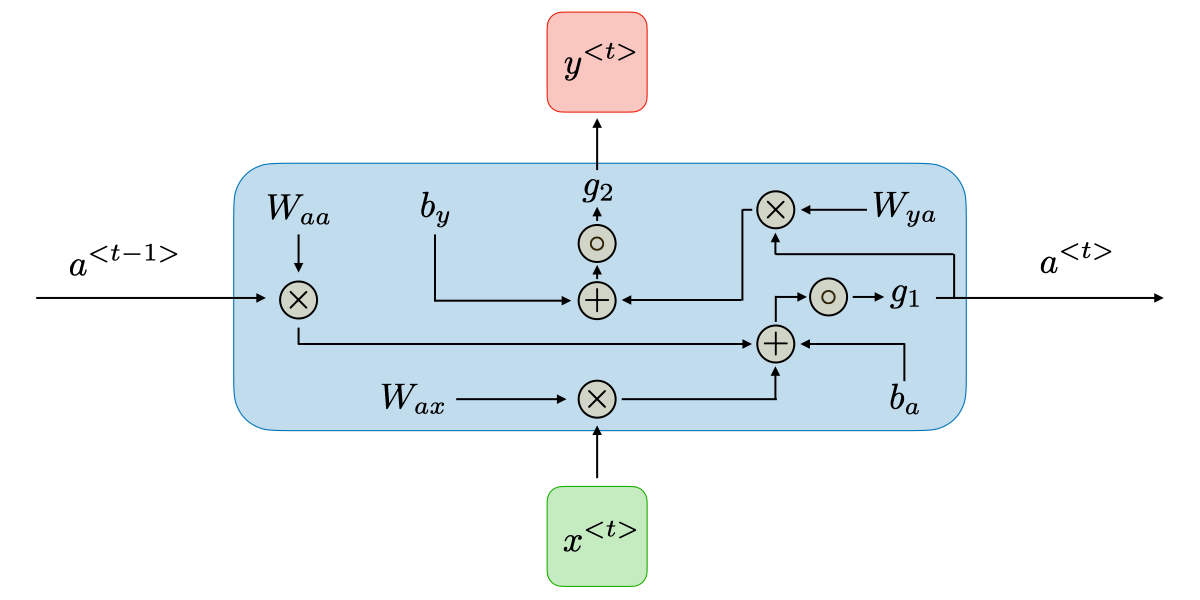
\includegraphics[width=\textwidth]{bibliography/Figure/RNNmodel.png}
        \caption{Architecture of a Traditional RNN}
        \label{fig:3}
\end{minipage}
\end{figure}
=======
>>>>>>> 24940c910db10766da1e8600f40dc6fa53ff0bdd

% UNCOMMENT these lines below (and remove the 2 commands above) if you want to embed the bibliografy.
\begin{thebibliography}{00}
\bibitem{cakra2015stock}
Yahya Eru Cakra and Bayu Distiawan Trisedya. "Stock price prediction using linear regression based on sentiment analysis." In: 2015 International Conference on Advanced Computer Science and Information Systems (ICACSIS). IEEE, 2015. pp. 147-154.
\bibitem{uras2020forecasting}
Nicola Uras, et al. "Forecasting Bitcoin closing price series using linear regression and neural networks models." PeerJ Computer Science, vol. 6, 2020, article e279.
\bibitem{dadhich2021predictive}
Manish Dadhich, et al. ``Predictive models for stock market index using stochastic time series ARIMA modeling in emerging economy.'' In: Advances in Mechanical Engineering: Select Proceedings of CAMSE 2020. Springer Singapore, 2021. pp. 281-290.
\bibitem{garlapati2021stock}
Anusha Garlapati, et al. ``Stock price prediction using Facebook Prophet and ARIMA models.'' In: 2021 6th International Conference for Convergence in Technology (I2CT). IEEE, 2021. pp. 1-7.
\bibitem{ZhuRNN}
Zhu Y. Stock price prediction using the RNN model. InJournal of Physics: Conference Series 2020 Oct 1 (Vol. 1650, No. 3, p. 032103). IOP Publishing. 
\bibitem{DingGRU}
Ding X, Zhang Y, Liu T, Duan J. Deep learning for event-driven stock prediction. InTwenty-fourth international joint conference on artificial intelligence 2015 Jun 25.
\bibitem{ShejulGRU}
Shejul, A.A., Chaudhari, A., Dixit, B.A., Lavanya, B.M. (2023). Stock Price Prediction Using GRU, SimpleRNN and LSTM. In: Kulkarni, A.J., Mirjalili, S., Udgata, S.K. (eds) Intelligent Systems and Applications. Lecture Notes in Electrical Engineering, vol 959. Springer, Singapore 

\bibitem{fjellstrom2022lstm}
Carmina Fjellström. "Long Short-Term Memory Neural Network for Financial Time Series." arXiv:2201.08218v1 [q-fin.ST], 20 Jan 2022.
\bibitem{mehtab2020stock}
Sidra Mehtab and Jaydip Sen. "Stock Price Prediction Using CNN and LSTM-Based Deep Learning Mode." Department of Data Science, Praxis Business School, Kolkata, INDIA. Accepted version of paper presented at 2020 International Conference on Decision Aid Sciences and Applications (DASA’20), Bahrain, November 8 – 9, 2020.

\bibitem{ChenFFT}
Chen MY, Chen BT. Online fuzzy time series analysis based on entropy discretization and a Fast Fourier Transform. Applied Soft Computing. 2014 Jan 1;14:156-66. 

\bibitem{jin2019using}
Qingwen Jin, Xiangtao Fan, Jian Liu, Zhuxin Xue, and Hongdeng Jian. "Using eXtreme Gradient BOOSTing to Predict Changes in Tropical Cyclone Intensity over the Western North Pacific." Atmosphere, vol. 10, no. 6, 2019, pp. 341–.
\bibitem{chen2016xgboost}
Tianqi Chen (University of Washington) and Carlos Guestrin (University of Washington). "XGBoost: A Scalable Tree Boosting System."
\bibitem{nabiee2023stock}
Shima Nabiee and Nader Bagherzadeh. "Stock Trend Prediction: A Semantic Segmentation Approach." arXiv preprint arXiv:2303.09323, 2023.


% IV
\bibitem{Gillian}
Gillian Smith, " The Fast Fourier Transform and its Applications ", \url{https://www.maths.ed.ac.uk/~ateckent/vacation_reports/summer_project_gillian_smith.pdf}, Accessed August 2019. 
<<<<<<< HEAD


% FFT
\bibitem{Gillian}
Gillian Smith, " The Fast Fourier Transform and its Applica-
tions ",\url{ https://www.maths.ed.ac.uk/~ateckent/vacation_reports/summer_ project_gillian_smith.pdf}, Accessed August 2019.

\bibitem{Musbah}
Musbah, H., El-Hawary, M., \& Aly, H. (2019). Identifying Seasonality in
Time Series by Applying Fast Fourier Transform. 2019 IEEE Electrical
Power and Energy Conference (EPEC).

\bibitem{Roberts}
S.J. Roberts. "Lecture 7 - The Discrete Fourier Transform". Available at:
\url{https://www.robots.ox.ac.uk/~sjrob/Teaching/SP/l7.pdf}. Accessed: 2000.

\bibitem{busin}
Evans, J. R., *Business Analytics: Methods, Models, and Decisions*. Hoboken, NJ: Wiley, 2013, p. 276.

\bibitem{Xgboost}
T. Chen and C. Guestrin, "XGBoost: A Scalable Tree Boosting System," arXiv:1603.02754v3 [cs.LG], June 10, 2016.

\bibitem{geekXGboost}
P. Pawangfg, "XGBoost," GeeksforGeeks, Available: https://www.geeksforgeeks.org/xgboost/. [Accessed: 06-Feb-2023].

%GRU
\bibitem{Yamak}
Yamak, P. T., Yujian, L., \& Gadosey, P. K. (2019, December). A comparison between arima, lstm, and gru for time series forecasting. In Proceedings of the 2019 2nd international conference on algorithms, computing and artificial intelligence (pp. 49-55).
%FCN
\bibitem{Ismail}
Ismail Fawaz, H., Forestier, G., Weber, J., Idoumghar, L., \& Muller, P. A. (2019). Deep learning for time series classification: a review. Data mining and knowledge discovery, 33(4), 917-963.
% RNN
\bibitem{IBM}
IBM Technology company, “What are recurrent neural networks?”, Available at: \url{https://www.ibm.com/topics/recurrent-neural-networks}
\bibitem{Chung}
Chung, Junyoung, Caglar Gulcehre, KyungHyun Cho, and Yoshua Bengio. "Empirical evaluation of gated recurrent neural networks on sequence modeling." arXiv preprint arXiv:1412.3555 (2014).
\bibitem{standford}
A. Amidi and S. Amidi, "Recurrent Neural Networks Cheatsheet," Stanford University, [Online]. Available: \url{https://stanford.edu/~shervine/teaching/cs-230/cheatsheet-recurrent-neural-networks}. [Accessed: 29-May-2024]. 

=======
>>>>>>> 24940c910db10766da1e8600f40dc6fa53ff0bdd


% FFT
\bibitem{Gillian}
Gillian Smith, " The Fast Fourier Transform and its Applica-
tions ",\url{ https://www.maths.ed.ac.uk/~ateckent/vacation_reports/summer_ project_gillian_smith.pdf}, Accessed August 2019.

\bibitem{Musbah}
Musbah, H., El-Hawary, M., \& Aly, H. (2019). Identifying Seasonality in
Time Series by Applying Fast Fourier Transform. 2019 IEEE Electrical
Power and Energy Conference (EPEC).

\bibitem{Roberts}
S.J. Roberts. "Lecture 7 - The Discrete Fourier Transform". Available at:
\url{https://www.robots.ox.ac.uk/~sjrob/Teaching/SP/l7.pdf}. Accessed: 2000.

\bibitem{busin}
Evans, J. R., *Business Analytics: Methods, Models, and Decisions*. Hoboken, NJ: Wiley, 2013, p. 276.

\bibitem{Xgboost}
T. Chen and C. Guestrin, "XGBoost: A Scalable Tree Boosting System," arXiv:1603.02754v3 [cs.LG], June 10, 2016.

\bibitem{geekXGboost}
P. Pawangfg, "XGBoost," GeeksforGeeks, Available: https://www.geeksforgeeks.org/xgboost/. [Accessed: 06-Feb-2023].

%GRU
\bibitem{Yamak}
Yamak, P. T., Yujian, L., & Gadosey, P. K. (2019, December). A comparison between arima, lstm, and gru for time series forecasting. In Proceedings of the 2019 2nd international conference on algorithms, computing and artificial intelligence (pp. 49-55).
%FCN
\bibitem{Ismail}
Ismail Fawaz, H., Forestier, G., Weber, J., Idoumghar, L., \& Muller, P. A. (2019). Deep learning for time series classification: a review. Data mining and knowledge discovery, 33(4), 917-963.
\end{thebibliography}




%%%%%%%%%%%%%%%


\EOD

\end{document}
